\documentclass[12pt]{article}
\def\title{Final Project}
\def\course{MNXB11}
\usepackage[a4paper, margin=0.95in]{geometry}
\usepackage{amsmath,amsthm,amsfonts,amssymb,mathrsfs,comment,scalerel,graphicx,tabularx,systeme,mathtools,float,svg,hyperref,pgf,multirow,xcolor,footnote,caption,subcaption,listings,indentfirst,wrapfig,siunitx,lmodern,parskip,tabularray,longtable}
\usepackage[section]{placeins}
\usepackage[framemethod=TikZ]{mdframed}
\usepackage[title]{appendix}
\usepackage[nottoc]{tocbibind}
\usepackage[most]{tcolorbox}

\usepackage[utf8]{inputenc}
\setcounter{tocdepth}{2}
\numberwithin{equation}{section}
\renewcommand{\theequation}{Eq. \thesection.\arabic{equation}} 
\usepackage[style = numeric-comp,
backend=biber, autocite = superscript]{biblatex}
\addbibresource{bibliography.bib}
\newcommand{\filename}[1]{\texttt{\detokenize{#1}}}
\definecolor{codegreen}{RGB}{0,120,70}
\definecolor{codegray}{RGB}{100,100,100}
\definecolor{codeblue}{RGB}{30,70,160}
\definecolor{codebackground}{RGB}{245,245,245}
\lstset{
    basicstyle=\ttfamily\small,
    backgroundcolor=\color{codebackground},
    commentstyle=\color{codegreen},
    keywordstyle=\color{codeblue}\bfseries,
    stringstyle=\color{red!70!black},
    numbers=left,
    numberstyle=\tiny\color{codegray},
    numbersep=8pt,
    breaklines=true,
    breakatwhitespace=false,
    frame=single,
    rulecolor=\color{codegray!40},
    tabsize=4,
    showstringspaces=false,
    captionpos=b
}

\hypersetup{
    colorlinks=true,
    linkcolor=blue,
    filecolor=magenta,      
    urlcolor=cyan,
    citecolor=cyan,
    pdftitle={\title }}

\newtcbtheorem[auto counter,number within=section]{def-box}%
  {Defintion}{fonttitle=\bfseries\upshape, fontupper=\slshape,
     arc=0mm, colback=blue!5!white,colframe=blue!75!black}{definition}




% The document Starts here.


\begin{document}

\begin{titlepage}
    \newcommand{\HRule}{\rule{\linewidth}{0.5mm}}
    
    \centering
    \textsc{\LARGE \course}\\[2cm]
    
    \HRule\\[1cm]
    {\huge\bfseries \title}\\[0.4cm]
    \HRule\\[1.5cm]
    
    \begin{minipage}{0.5\textwidth}
        \centering
        \large
        \textit{Author(s)}\\[0.5cm]
        Charlotte Rösler  \\ 
        Herman Plank \\
        Love Hagerberg  \\ 
        Samuel Kattaya \\[0.5cm]
    \end{minipage}
    
    \vfill
    
    \includesvg[width=0.4\textwidth]{lundlogo.svg}
    
    \vfill
    {Hand-in Date: \today}
    
    \vfill
\end{titlepage}



{\hypersetup{linkcolor=black} \tableofcontents}
\newpage

\section{Introduction}


\section{Numerical Methods}

\subsection{Cleaning of Raw Data}
The data was cleaned in bash. The bash program takes the .txt data in and splits the columns into year, month, day, hour, minute, second, temperature and grading. This is done, so that all data is clearly identified in later stages of the analysis. All comments are taken are not taken into account. Finally the bash program creates a \filename{cleaned_filename.csv} in the datasets directory with measurements in the format   \texttt{YYYY-MM-DD HH:MM:SS Temperature Y/G} . 

\subsection{Creating a Root Tree}
The file \filename{src/run_weather.cxx} creates a root tree by accessing the specified csv file, separating the year, month, day, hour, minute, second, temperature and grading and writing each to a branch of the tree called \filename{MNXB11_Temperature} stored in a root-file called \filename{weather_data.root}. If there is data that is not correctly formatted, which means that numbers do not build valid dates and times, then the data is not written to the tree. Measurements before 1500 and after 2026 are also rejected.

\subsection{Making the Makefile}
In order to turn our written code into something that a machine can run we have to compile and link all of our different files, making a build. The instructions to do this are stored in the Makefile. \\

The first part of our Makefile (line 1-10) has some framework for the code. It establishes things like using the g++ compiler, which errors to flag for and what version of c++ we are using. Lines 7 and 8 make it so the program can compile with all the ROOT specific libraries and flags, which makes includes like TGraph possible. Line 10 puts everything under the variable CXXFLAGS which makes it easier to reference later. The Makefile declares that the target 'all' is dependent on main in line 17. This does two things: It makes sure that the file exists before proceeding and it checks if the file is up-to-date, this means main doesn't get remade unnecessarily if nothing has changed since the last time make was run. Makefile then proceeds to do four things:
\begin{itemize}
    \item Create a dictionary so that ROOT can interpret our 'measurement' class that was written in c++. Most important to note is the 'rootcling' command which makes it so the program looks in our LinkDef header for instructions on when and how to make a library. 
    \item Compiling all of our source files and the library using a pattern rule for the source files in lines 32-33.
    \item Building a shared library by linking our files that pertain to the data as well as the newly created ROOT dictionary through a file called libMNXB11.so. Technically, for the purposes of this project a static library would work just as well. The shared library implementation is an artifact of an earlier stage in the project when we had several different macros that could be run independently rather than having all the analysis be done through one executable like now.
    \item Linking the analysis files and the library into the executable main. Separating the library-linking from the file-linking by using (filter \%.o,\^ ).
\end{itemize}

\subsection{Making Main Flexible}
The main.cxx isn't just a list of our commands. It takes two arguments, the command itself and the name of a city. This name is then given further as an argument to the functions that need it meaning with just one command you can get the analysis of any of the datasets. 


\section{Analytical Methods}

\subsection{Yearly Average}
The yearly average is found by taking the mean over all measurement points during one year. If the year has no measurements it is excluded from the measurements and not considered in further calculations. The same is done for years that have an unequal distribution of measurement points during the year, which is evaluated by looking at the number of measurement points per month and allowing measurements for which the difference between the maximum and minimum measurement points per month and year is smaller than $1/3$ of the maximum points.\\
The mean over the whole measurement period is calculated with all years with valid mean temperatures.
The running average is calculated over a period of $\pm 10$ years from the center year. If there were years with excluded or no measurements the running average was still computed but no data was included from those years.

\subsection{Daily Average}

To determine the average temperature for each day of all the years obtained from the SMHI dataset, we first use a method to convert each calendar date into a Day Of Year (DOY), and then use std::map to map in each temperature for each of the DOY.
As there are usually 4 readings for each date, we take the average of these readings for each of the DOY. Now we have a list of DOY with a mean temperature of each DOY for each of the years from the dataset. We plot their average to get the mean daily temperature and the standard deviation of each of the DOY.


\subsection{Extreme temperatures}

To extract yearly extreme temperatures from the datasets, the program first makes a guess that every year the max temp was -9999 $^o$C and min was 9999 $^o$C. It then goes through the entire data set entry by entry, first checking that the temperature isn't above or below $\pm 40 ~^o$C, to rule out values that are probable errors. It then compares if the stored min/max for the year is higher/lower than the current entry. If the entry is found to be a more extreme temperature, the old value is thrown out and replaced. The month that the new extreme value was recorded in is also saved for the plotting. The same is also done but for each month of the year to find the monthly extremes.

\subsection{Hottest and Coldest Days}

To present how often days of the year were hottest or coldest the program starts (in line 17-27) two lists that it can add to: The first contains tuples of the year, month, day, temperature and how many times the first three have appeared together. The second list contains tuples with a year, an integer place in a year and the average temperature. After receiving the data (line 43) the program proceeds to go through every day in the dataset, getting its year, month day and temperature. If the day appears again the count-value goes up and the temperature measurement gets added to the previous entrys' (line 54-63). It goes on to group each entry in list one by year, average the entrys' temperatures, converting it to an integer value in the year and adding it into list two (lines 66-88). For each year it goes through every day and assigns it the hottest or coldest tag depending on if it is hotter/colder than the day currently marked as hottest/coldest in that year, before the first day the hottest temperature is negative infinity, the opposite for the coldest (lines (lines 95-113). Finally, it counts how many times the integer of a day has been tagged as hottest/coldest which can then be displayed (lines 116-125).

\section{Result and Analysis}

\subsection{Yearly Average}
The yearly average from Lund is portrayed in figure \ref{fig:yearly_avg_lund}. It shows that the mean temperature over the whole measurement period was $T=8$°C and is shown as the dashed line. The running average over 21 years is portrayed as the black line. Some histogram bins are not filled and instead show a gray background, because they did not fulfill the analysis requirements as described above.
\begin{figure}[H]
    \centering
    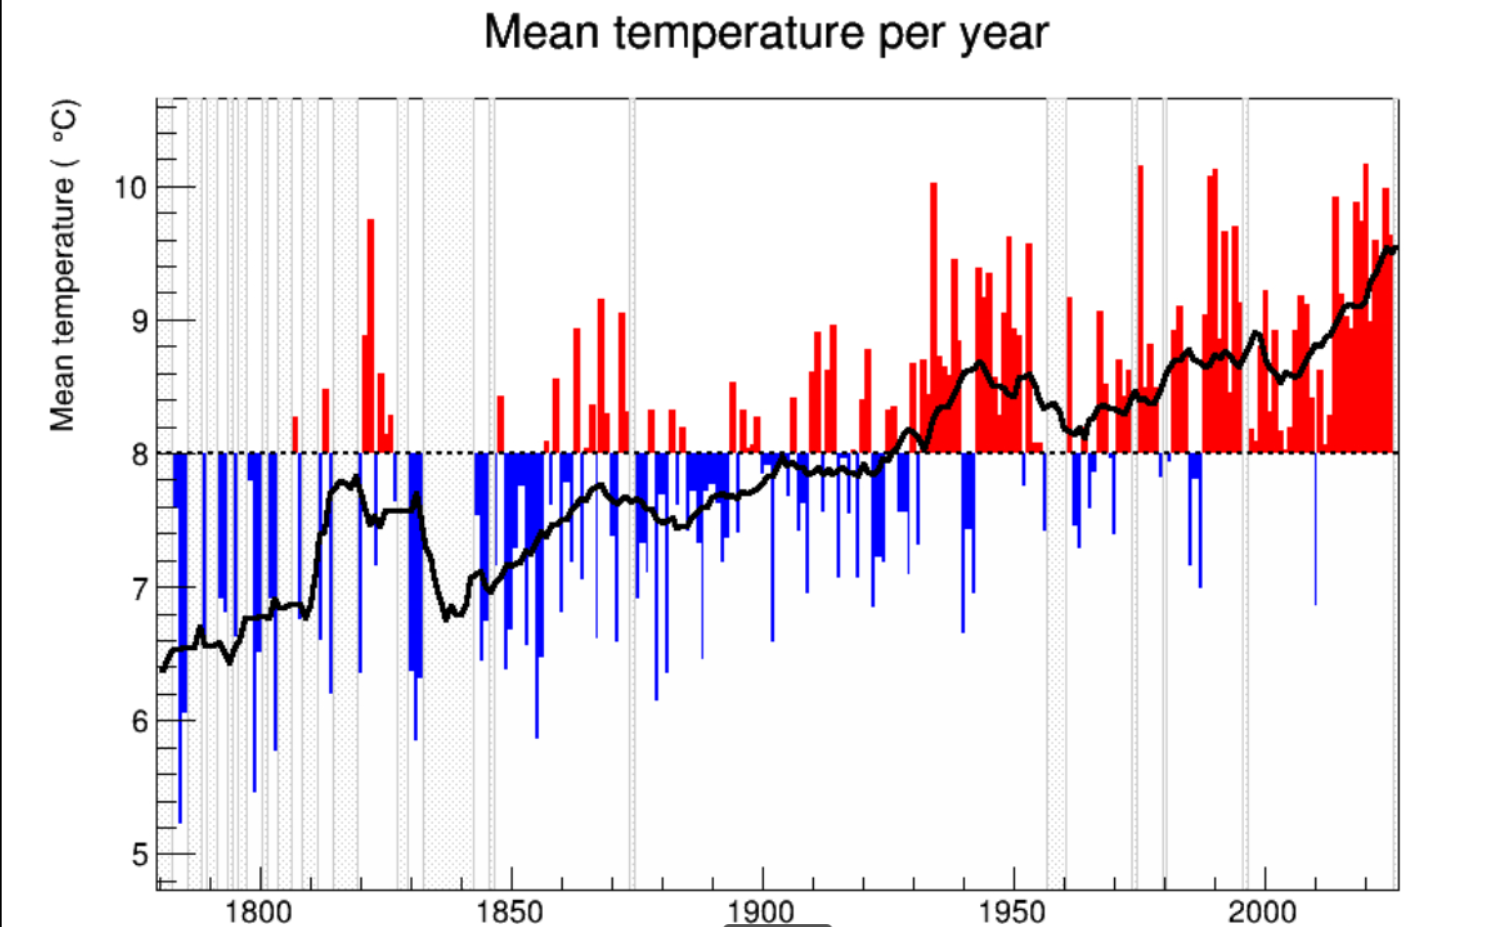
\includegraphics[width=0.75\linewidth]{Report/Avg_Yearly_Temp_Lund.png}
    \caption{The mean annual temperature in Lund with running average and overall mean temperature.}
    \label{fig:yearly_avg_lund}
\end{figure}
The running average increases over the 200 years by around 3 °C. In the beginning of the measurement period most average temperatures lie below the average. Then the average temperature increases and today most of the temperatures lie above the longtime mean.\\

\begin{figure}[H]
    \centering
    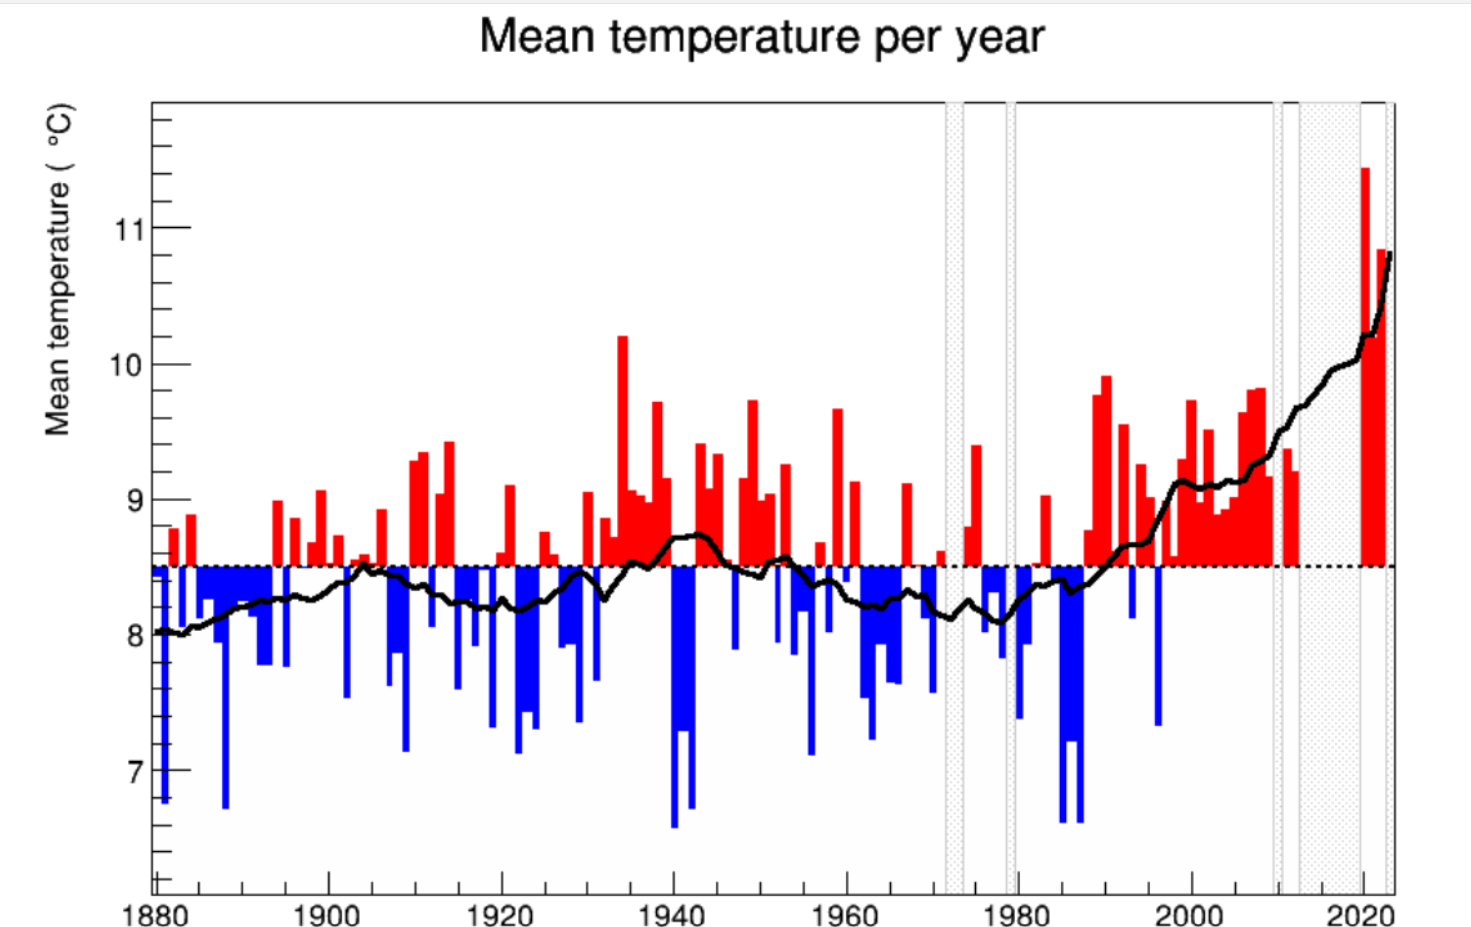
\includegraphics[width=0.75\linewidth]{Avg_Yearly_Temp_Falsterbo.png}
    \caption{The mean annual temperature in Falsterbo with running average and overall mean temperature.}
    \label{fig:yearly_avg_falsterbo}
\end{figure}

\subsection{Daily Average}

The seasonal cycle resembles a sinusoidal function, it is coldest at the start of the year during winter and increases toward the peak the middle of the year during summer, as seen in Figure \ref{fig:daily_avg_lund}.

\begin{figure}[H]
    \centering
    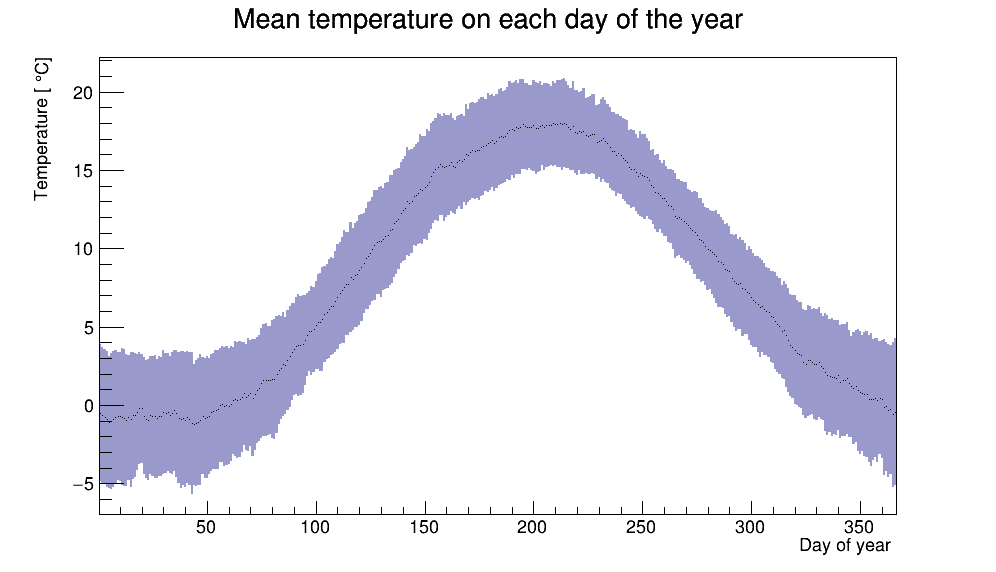
\includegraphics[width=0.75\linewidth]{Report/daily_average_temperature.png}
    \caption{The mean daily temperature in Lund on each day of the year, and its standard deviation.}
    \label{fig:daily_avg_lund}
\end{figure}

\subsection{Extreme temperatures}

\autoref{fig:yearly_extremes} and \autoref{fig:diff} show the results from looking at extreme temperatures in the Lund 1760-2026 dataset. Some years of data seems to be missing around 1955. We can in \autoref{fig:yearly_extremes} see that the extreme heat stays quite consistent over the years. However, the extreme cold seems to have a slight trend upwards in temperature.
This is reflected in \autoref{fig:year_diff}, which shows the temperature difference between the warmest and coldest day on average shrinking. We can see a similar trend in the difference in monthly extreme temperatures, shown in \autoref{fig:month_diff}, suggesting that our months may are becoming more "stable" in temperature.

\begin{figure}
    \centering
    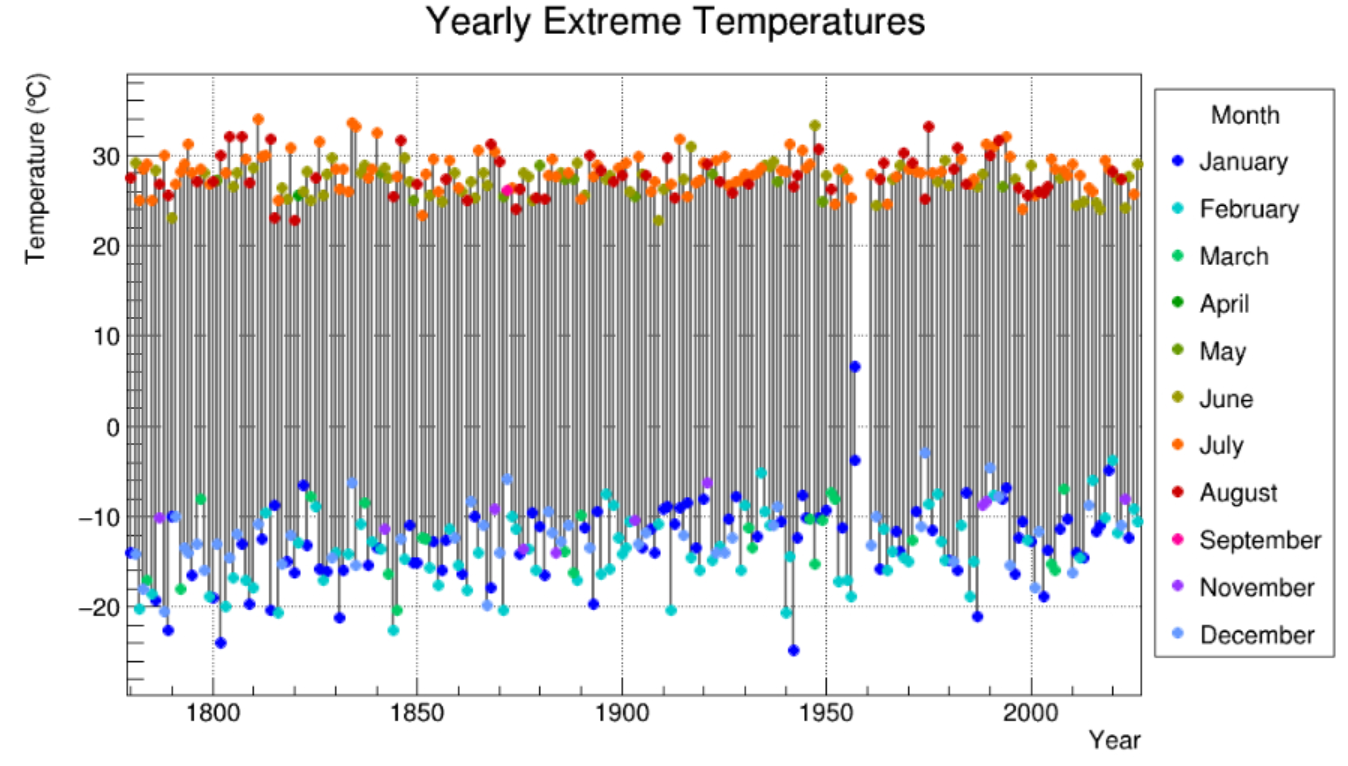
\includegraphics[width=0.7\linewidth]{Report/yearly_extremes.png}
    \caption{Yearly extremes recorded in Lund between 1760-2026. The color of a point relates to the month of the measurement. The vertical lines connect the coldest and hottest measurement of the year for readability.}
    \label{fig:yearly_extremes}
\end{figure}


\begin{figure}
\centering
\begin{subfigure}{.5\textwidth}
  \centering
  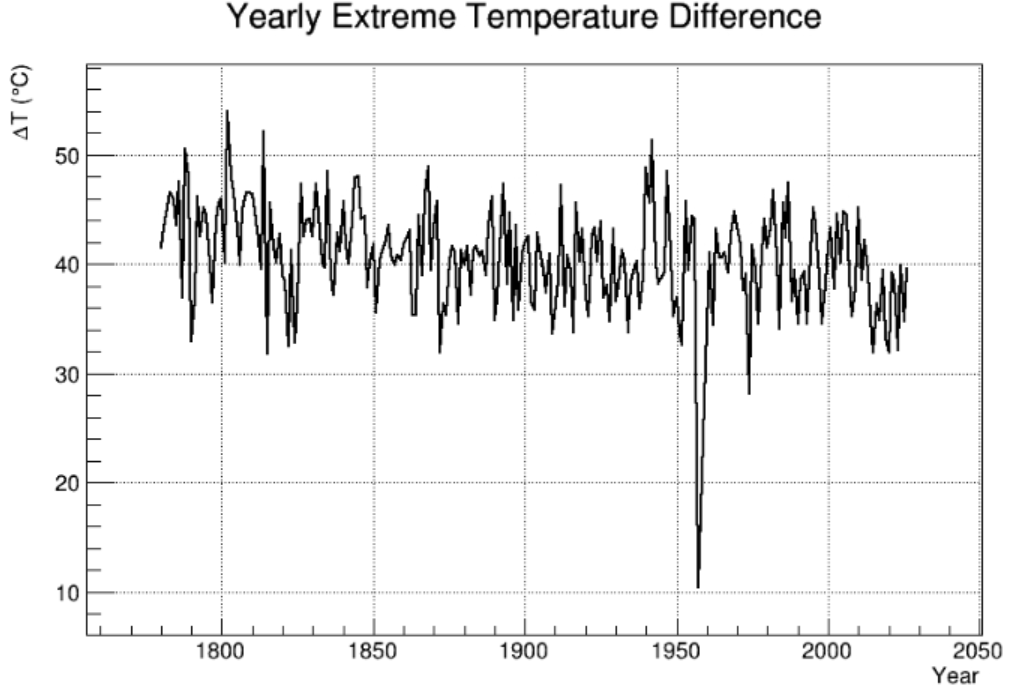
\includegraphics[width=.95\linewidth]{Report/yearly_diff.png}
  \caption{Difference between hottest and coldest measurements each year.}
  \label{fig:year_diff}
\end{subfigure}%
\begin{subfigure}{.5\textwidth}
  \centering
  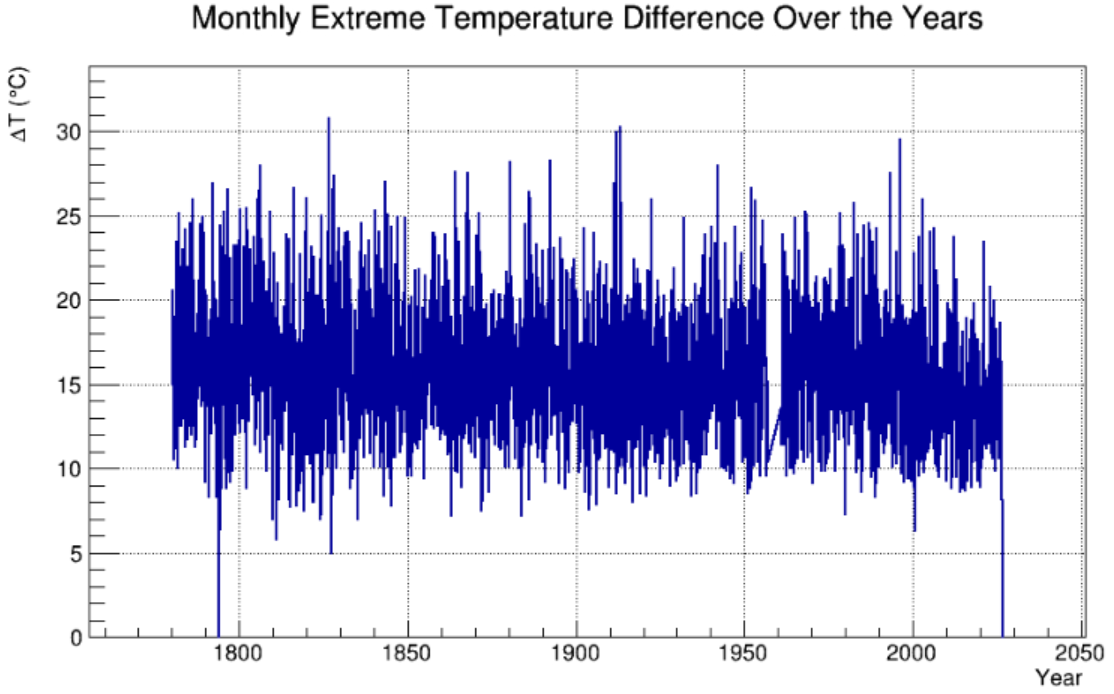
\includegraphics[width=1\linewidth]{Report/monthly_diff.png}
  \caption{Difference between hottest and coldest measurements each month.}
  \label{fig:month_diff}
\end{subfigure}
\caption{Extreme temperature differences in Lund 1760-2026.}
\label{fig:diff}
\end{figure}

\subsection{Hottest and Coldest Days}
\autoref{fig:Extremeyear} shows a distribution of hottest and coldest days which suggests that days in the middle of the year, between day 150 and 250, are more likely to be the hottest while days at the beginning or end of the year, day 325-75, are more likely to be coldest. Darker shades of colour indicate several days in close proximity that have had the same amount of extreme days. The day with the most amount of hot days at 10 is around 190, late June/early July, while the day with the most amount of cold at 8 is around 40, early/mid February.
\begin{figure}[H]
    \centering
    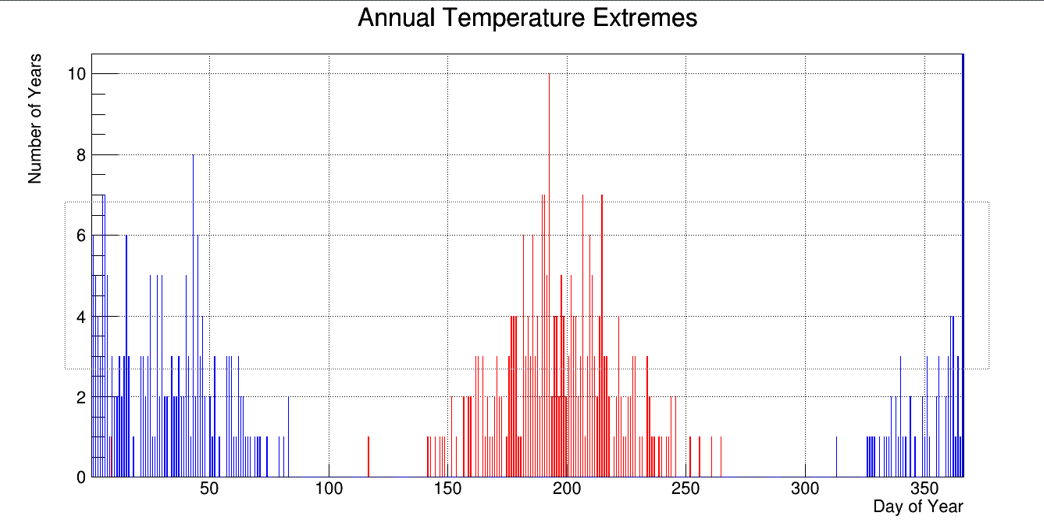
\includegraphics[width=0.75\linewidth]{Report/Annual_Temp_Ex_Lund.png}
    \caption{The amount of times a day in the year has be the hottest or coldest.}
    \label{fig:Extremeyear}
\end{figure}

\section{Discussion}

\subsection{Yearly Average}
The results for Lund and Falsterbo agree with the findings of SMHI that compared with 1890 the temperatures have been raised by 1.9°C on average \cite{SMHI_1}.Moreover, agree both measurements with each other showing a consistent picture of the climate developments in Skåne. Both show a big increase of the running average in the last 40 years. Both plots show the same behavior considering that the mean temperature in Falsterbo is $0.5$°C higher than in Lund, because the data starts 100 years later.


\subsection{Daily Average}

The shaded band in Figure \ref{fig:daily_avg_lund} shows that the mean temperature fluctuates by about 4-5 $^oC$. It could be due to natural weather changes from one year into another, however some of it could come from using the both of the G and Y data quality grades, as well as missing data points or sensor location changes over time.


\subsection{Extreme temperatures}

It is hard to draw any real conclusions from the extracted data, but it suggests that Lund's winters are becoming warmer on average, while the hottest days during summer still are around the same temperature. However, since the mean yearly temperature is increasing, we can conclude that our summer days are getting hotter average temperatures, but not extremes. Looking at \autoref{fig:diff} we can see that our years and months might are becoming less extreme, but again it is difficult to know if we are seeing actual trends.

\subsection{Hottest and Coldest Days}

\autoref{fig:Extremeyear} presents as a probability curve and matches what we would expect. Winter is usually coldest and summer is usually hottest, with days in the middle of their respective season being at the extreme more often. 

There are some issues however. Primarily, the quality of the data collected. The original datasets list has data being listed as either 'G' or 'Y' for 'good' or 'subpar' without explaining where the lines go between categories. Excluding all the data marked 'Y' would remove hundreds of years from the analysis and could make it skew in strange ways as there could be years where only one seasons data was marked as 'G'. On top of this there are many completely missing days in the dataset that could make the graph non-representative. This is likely the cause of, for example, the one red line that is present at the beginning of the year. A future study would need better data to analyze.

Furthermore, it is somewhat hard to understand the data intuitively for this analysis. It would perhaps be better to group days into sections rather than having the individual days since, when initially viewing the diagram, it becomes natural to focus on the days with the most individual counts rather than how many consecutive days have a moderate or small amount of being the extreme case, which could be a better indicator of the distribution. Why certain individual days become the most frequent would need also further investigation.

\section{Conclusion}

\newpage

\defbibheading{bibintoc}[\refname]{
  \section{#1}   
}
\printbibliography[
heading=bibintoc ,
title={References}
]
\newpage
\section{Appendix} 

\end{document}